\documentclass{standalone}
\usepackage{circuitikz}
\begin{document}
	% Insert figure here
    	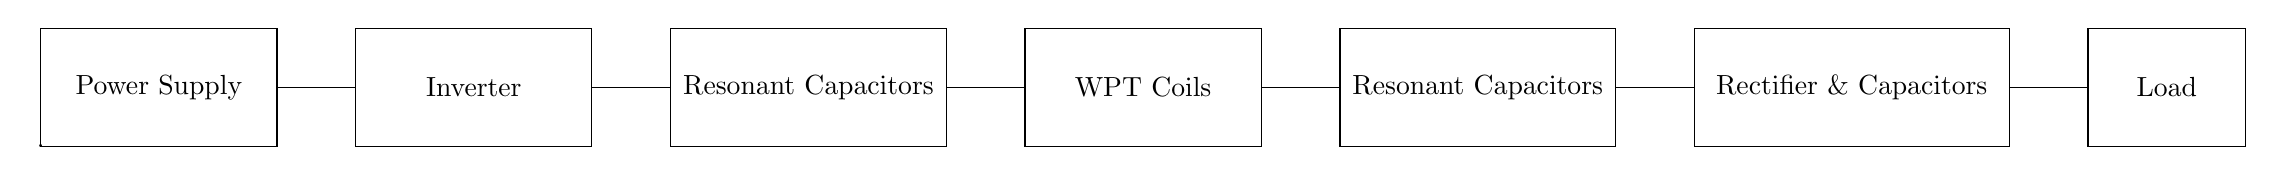
\begin{tikzpicture}
    
    \draw (0,0) node{.};
\draw  (0,1.5) rectangle (3,0) node[midway]{Power Supply};
\draw  (4,1.5) rectangle (7,0)node[midway]{Inverter};
\draw  (8,1.5) rectangle (11.5,0) node[midway]{Resonant Capacitors};
\draw  (12.5,1.5) rectangle (15.5,0) node[midway]{WPT Coils};
\draw  (16.5,1.5) rectangle (20,0) node[midway]{Resonant Capacitors};
\draw  (21,1.5) rectangle (25,0) node[midway]{Rectifier \& Capacitors};
\draw  (26,1.5) rectangle (28,0) node[midway]{Load};
\draw (3,0.75) -- (4,0.75) node (v1) {} -- (v1) -- cycle;
\draw (7,0.75) -- (8,0.75) node (v2) {} -- (v2) -- cycle;
\draw (11.5,0.75) -- (12.5,0.75) node (v3) {} -- (v3) -- cycle;
\draw (15.5,0.75) -- (16.5,0.75) node (v4) {} -- (v4) -- cycle;
\draw (20,0.75) -- (21,0.75) node (v5) {} -- (v5) -- cycle;
\draw (25,0.75) -- (26,0.75) node (v6) {} -- (v6) -- cycle;
\end{tikzpicture}
\end{document}